\subsection{User Input}
\label{sub:user_input}

In order to present a user with useful information, our application will have
to accept data from them. This is done by means of forms, text input and
buttons. To maintain a clean, intuitive user interface, a simplistic approach
is often taken to reduce the thinking time required to process information on a
single screen. If more information is required, multiple screens are often
used.

\subsubsection{Timetables}
\label{ssub:timetables}

A common set of information presented to a user which represents a considerable
challenge, particularly on small screens, is a timetable of available or
appropriate times. From this, the user can then select which is most suitable
for them. When too much information is displayed on a single screen, this can
become confusing or impossible to read. For example, in
figure~\ref{fig:GoogleCalendarTimetable}\cite{GoogleCalendar}, despite a single
hour being a common appointment length, the text for these slots is hidden
entirely.
\begin{figure}[ht]
	\centering
	\begin{subfigure}[b]{0.25\textwidth}
		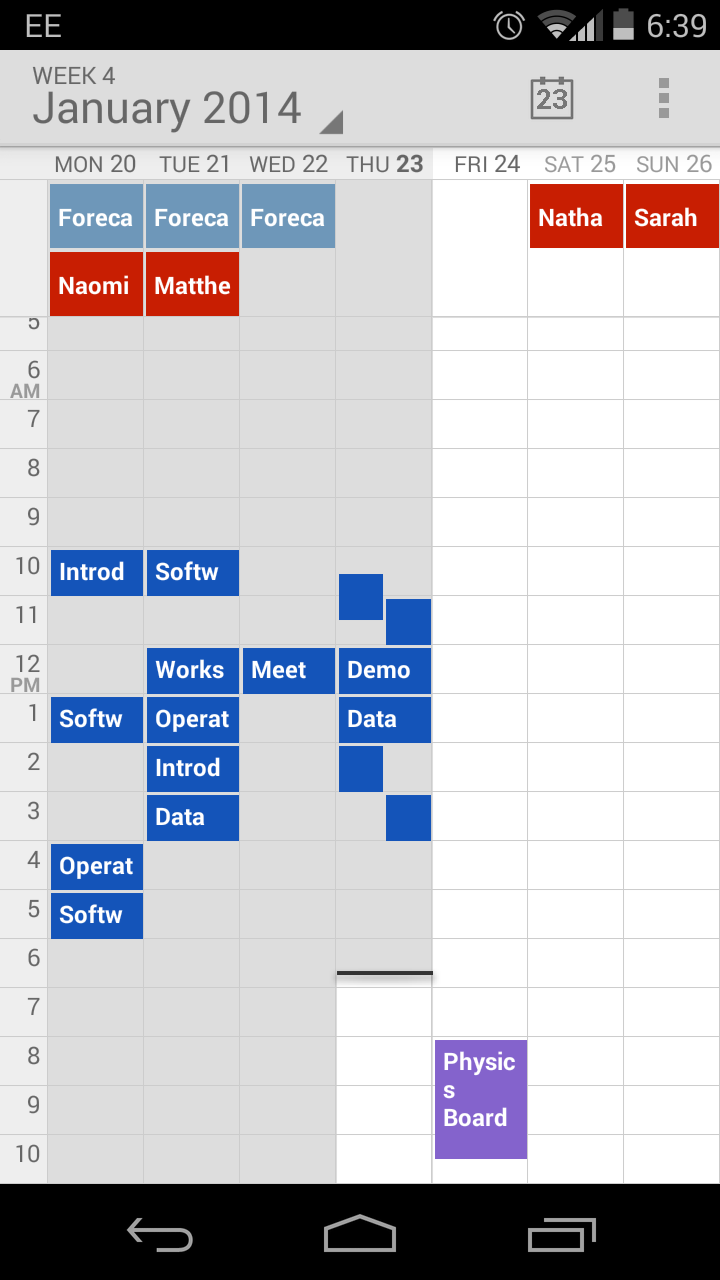
\includegraphics[width=\textwidth]{img/relatedReviews/GoogleCalendarTimetable.png}
		\caption{Google Calendar}\label{fig:GoogleCalendarTimetable}
	\end{subfigure}%
	\qquad
	\begin{subfigure}[b]{0.25\textwidth}
		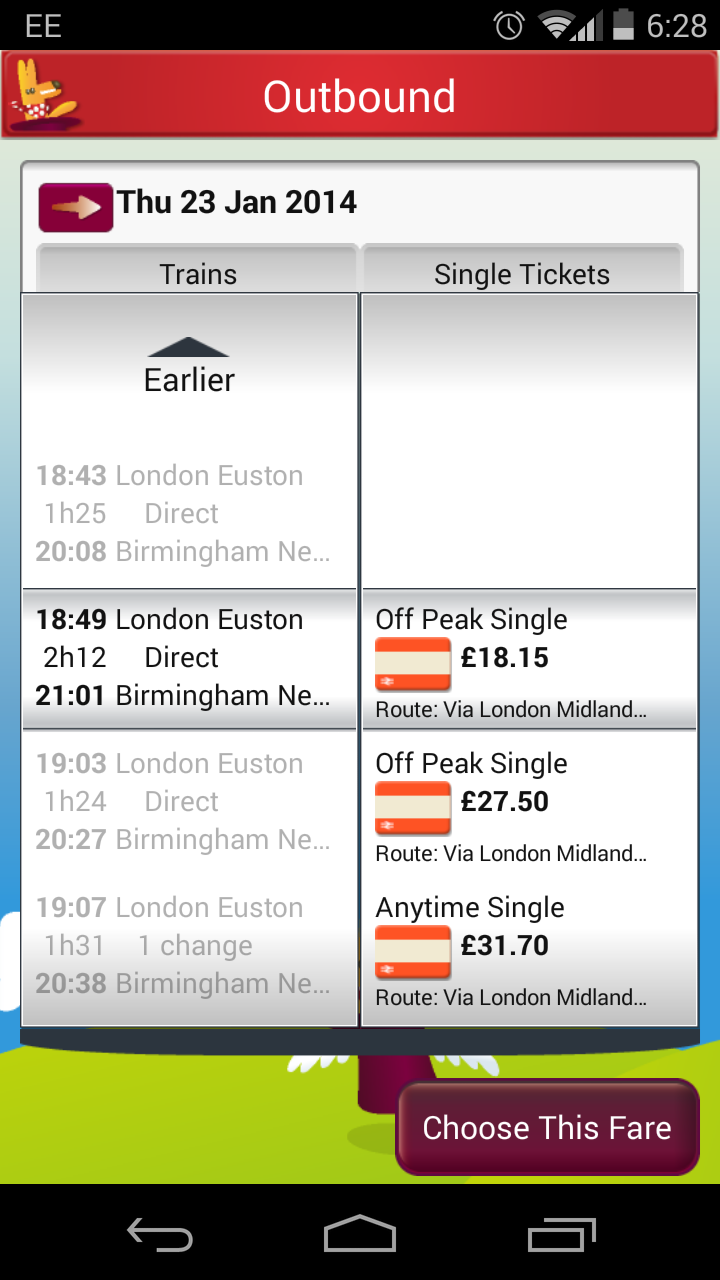
\includegraphics[width=\textwidth]{img/relatedReviews/RedSpottedHankyTicketSelection}
		\caption{RedSpottedHanky}\label{fig:RedSpottedHankyTicketSelection}
	\end{subfigure}
	\caption{When too much information is displayed on a screen, it can be
		hard to read and interpret, whereas condensing the information and
		splitting it so that only currently appropriate information is shown
	makes it much easier to understand. }\label{fig:timetables}
\end{figure}

A common way to improve the readability of theses complex structures, which
often contain a large quantity of data, is to have graded selection of that
data. In other words, where there is an option to refine a search to reduce the
data needed to be displayed, only the  immediately relevant information is
displayed, with simple navigation to other relevant data.

This method can be seen clearly in the RedSpottedHanky.com application,
figure~\ref{fig:RedSpottedHankyTicketSelection} when a user is searching for
tickets for a specific date and time. Although there may be many trains within
a narrow time gap, the application shows a small number of tickets with the
option to move either earlier or later. Each ticket time is also associated
with a number of options relating to ticket price. These are shown only for the
currently selected ticket time.

% subsubsection timetables (end)

\subsubsection{Date/Time Selection}
\label{ssub:date_time_selection}

In order to reduce the search range, often a date and/or time selection
dialogue is used. Figure~\ref{fig:date_time_selection} shows two different
implementations.

Figure~\ref{fig:RedSpottedHankyDateTime}, on the right is an example, again,
from RedSpottedHanky\cite{RedSpottedHanky}, which shows the time selection
associated with booking a train ticket. This design fails since the method of
changing time requires very close control when accuracy is required, and is
time consuming when the desired time is far from the currently selected time.
The movement is performed in single increments or decrements of the hours and
minutes. This is despite the functionality described above which lets the user
view and switch to other trains at nearby times.

Figures~\ref{fig:GoogleCalendarDateTime}, in the middle
and~\ref{fig:GoogleCalendarDateTime2} on the left are examples from Google
Calendar which shows how the process can be made much more intuitive, simple
and fast. Through the use of separate screens with large and clear selection,
this selection is much easier to navigate than the scrolling method used above.
\begin{figure}[ht]
	\centering
	\begin{subfigure}[b]{0.25\textwidth}
		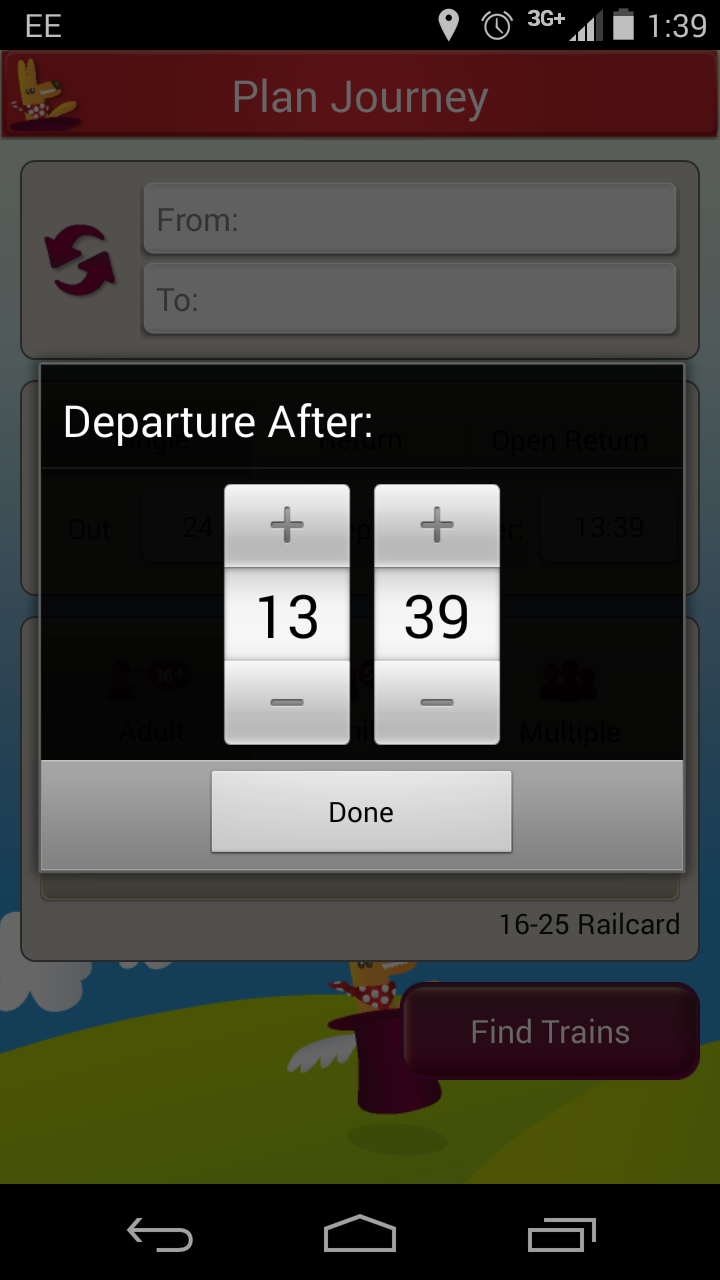
\includegraphics[width=\textwidth]{img/relatedReviews/RedSpottedHankyDateTime}
		\caption{RedSpottedHanky}\label{fig:RedSpottedHankyDateTime}
	\end{subfigure}%
	\qquad
	\begin{subfigure}[b]{0.25\textwidth}
		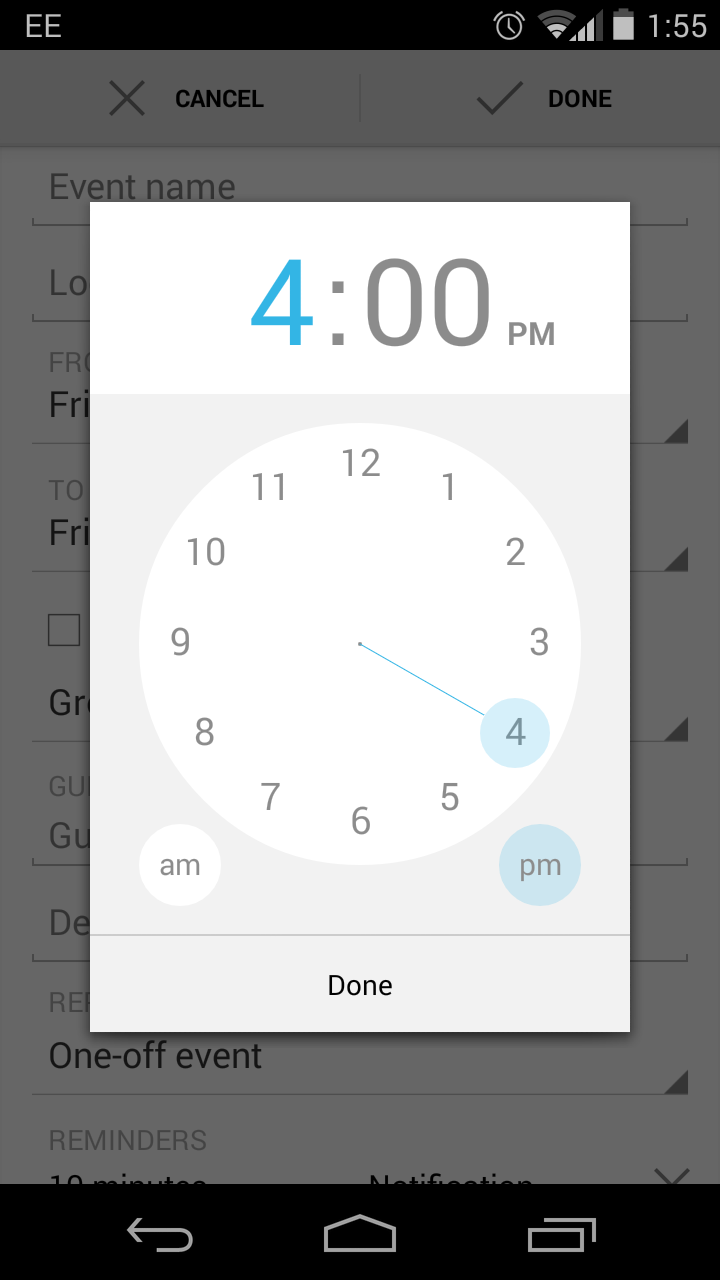
\includegraphics[width=\textwidth]{img/relatedReviews/GoogleCalendarDateTime}
		\caption{Google Calendar}\label{fig:GoogleCalendarDateTime}
	\end{subfigure}
	\qquad
	\begin{subfigure}[b]{0.25\textwidth}
		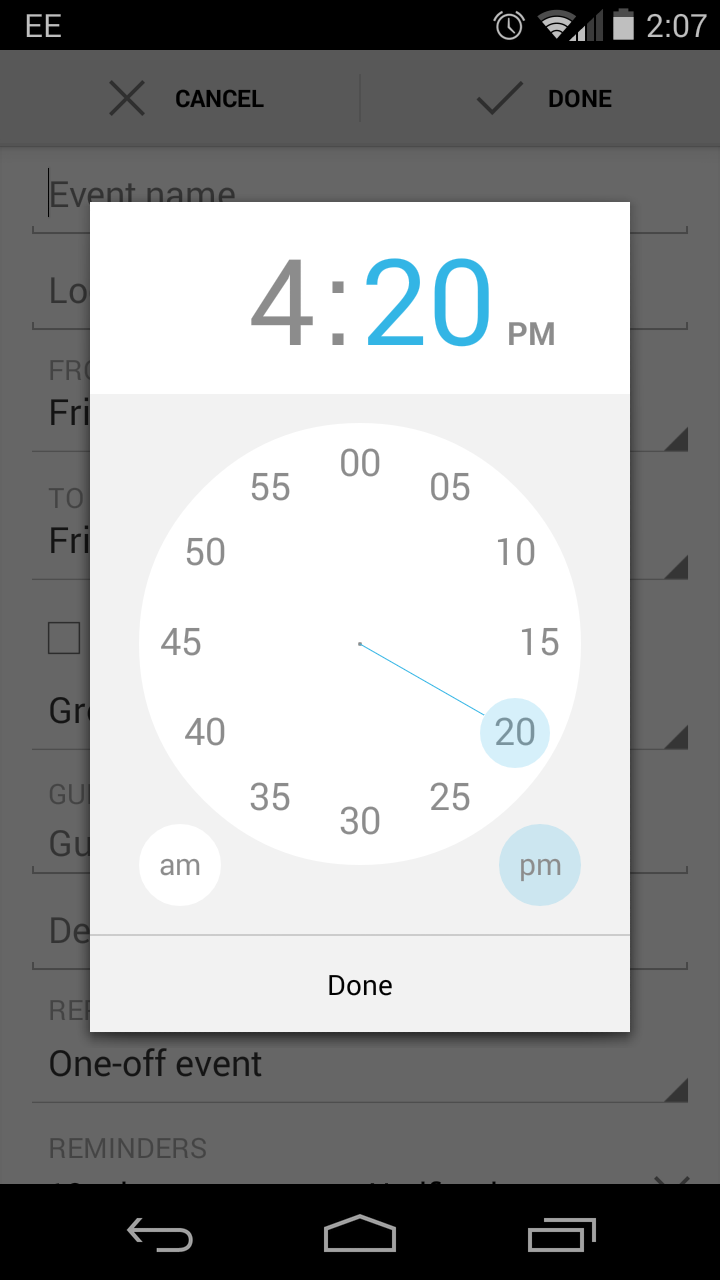
\includegraphics[width=\textwidth]{img/relatedReviews/GoogleCalendarDateTime2}
		\caption{Google Calendar}\label{fig:GoogleCalendarDateTime2}
	\end{subfigure}
	\caption{The time selection for RedSpottedHanky requires the user to
		spend to much time selecting the time when larger increments could be
		used to smoothen the process. Google Calendar, on the other hand,
		allows simple and fast selection of the hours and minutes through
	separate screens. }\label{fig:date_time_selection}
\end{figure}

A combination of both of these is used in the stock iOS, shown in
figure~\ref{fig:iOSDateTime}\cite{iOSDateTime} where a much easier to navigate
scrolling mechanism is used. Though this can still cause the user to spend more
time selecting the correct number, the fact that the used can ``flick scroll''
though the numbers means reaching a value that is far from the currently
selected one is much quicker than the RedSpottedHanky.com application.
\begin{figure}[ht]
	\centering
	\begin{subfigure}[b]{0.25\textwidth}
		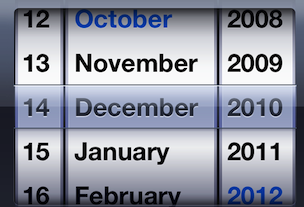
\includegraphics[width=\textwidth]{img/relatedReviews/iOSDateTime}
		\caption{RedSpottedHanky}
	\end{subfigure}%
	\qquad
	\begin{subfigure}[b]{0.35\textwidth}
		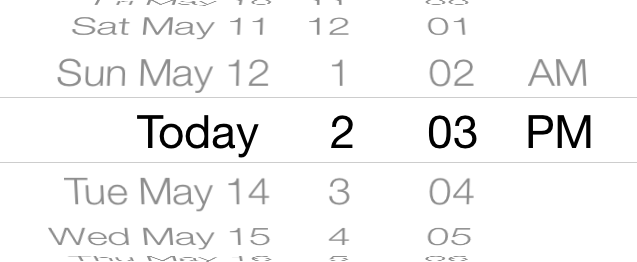
\includegraphics[width=\textwidth]{img/relatedReviews/iOS7DateTime}
		\caption{Google Calendar}
	\end{subfigure}
	\caption{Stock iOS date and time picker is easier to scroll through, but
		still requires more time than selecting the appropriate number.
	}\label{fig:iOSDateTime}
\end{figure}

% subsubsection date_time_selection (end)

\subsubsection{Forms}
\label{ssub:forms}

When entering information that is not limited to a small set of possible
values, such as a name, location or arbitrary number, a form must be used to
accept the user input. Since touch screens rely of the user being able to
navigate to to correct form section, the input must be of sufficient size to
allow this movement easily.

Figure~\ref{fig:TescoFormInput} show a simple form with two input boxes. Each
has a clear border around it so the target for interaction is easier to select.

An important consideration that has been made here is to specify that, for the
second set of text input, the data is strictly limited to digits. For this
reason, the keyboard switches from a general purpose ``qwerty'' keyboard to a
purely numerical version. Again, this assists the user, both by indicating that
only the provided digits are acceptable, and making the input of those digits
easier (often the numbers on a touch screen keyboard are only accessible by
switching modes).
\begin{figure}[ht]
	\centering
	\begin{subfigure}[b]{0.2\textwidth}
		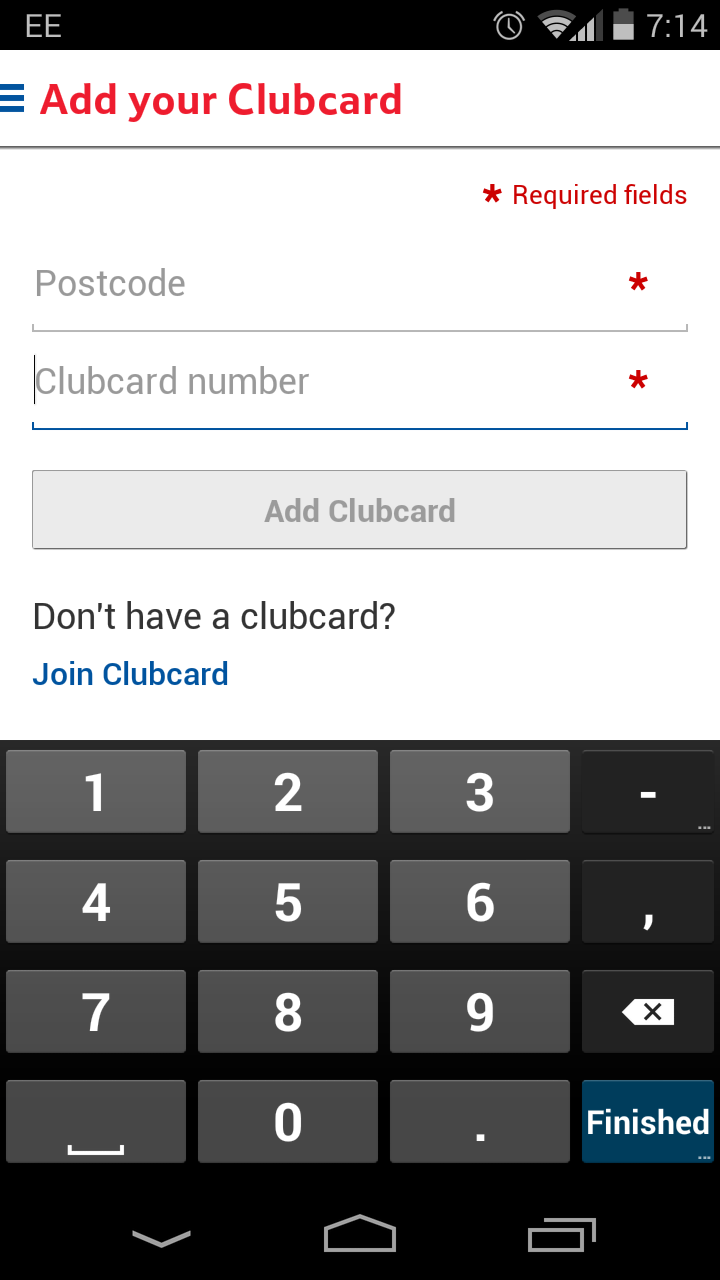
\includegraphics[width=\textwidth]{img/relatedReviews/TescoFormInput}
		\caption{Large, easy to access text entry}\label{fig:TescoFormInput}
	\end{subfigure}%
	\qquad
	\begin{subfigure}[b]{0.25\textwidth}
		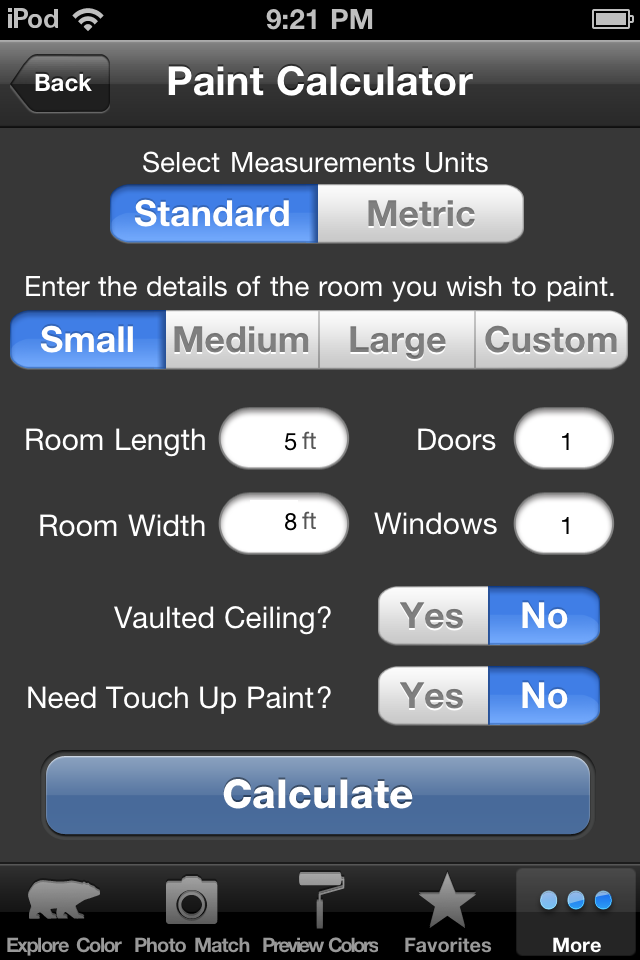
\includegraphics[width=\textwidth]{img/relatedReviews/PaintCalculatorCrowded}
		\caption{Crowded interfaces make entry more difficult.}
	\end{subfigure}
	\caption{}\label{fig:PaintCalculatorCrowded}
\end{figure}

By contrast, the interface in figure~\ref{fig:PaintCalculatorCrowded} is overly
crowded with too many small buttons squashed together. This could cause the
user to select the wrong input area, or not be able to navigate the application
properly.
% subsubsection forms (end)

% subsection user_input (end)
